\documentclass[a4paper,11pt,abstract=on,twoside,openright]{book}
\setlength\parindent{1.2em}

\usepackage[final=false]{../../common/naps62}

\newcommand{\common}[1]{\input{../../common/#1}}
\newcommand{\image}[4][]{%
  \begin{figure}[!htp]%
    \centering%
    \includegraphics[#1]{#2}%
    \caption{#3 \label{#4}}%
  \end{figure}
}

% include custom mathematical definitions
\common{equations/defs}

\hypersetup{pdfauthor={Miguel Branco Palhas}}
\hypersetup{pdftitle={Thesis: An Evaluation of the GAMA/StarPU Frameworks for Heterogeneous Platforms: The Progressive Photon Mapping Algorithm}}

\addbibresource{../../common/bib/parallel,../../common/bib/gama,../../common/bib/starpu,../../common/bib/gpu,../../common/bib/verbal,../../common/bib/photon_mapping}

% reduce chapter margins, only for scrbook
%\renewcommand{\chapterheadstartvskip}{\vspace*{-1.6\baselineskip}}

\begin{document}

\pdfbookmark{Cover}{cover}
\pagenumbering{roman}
% TODO acrescentar capa depois
%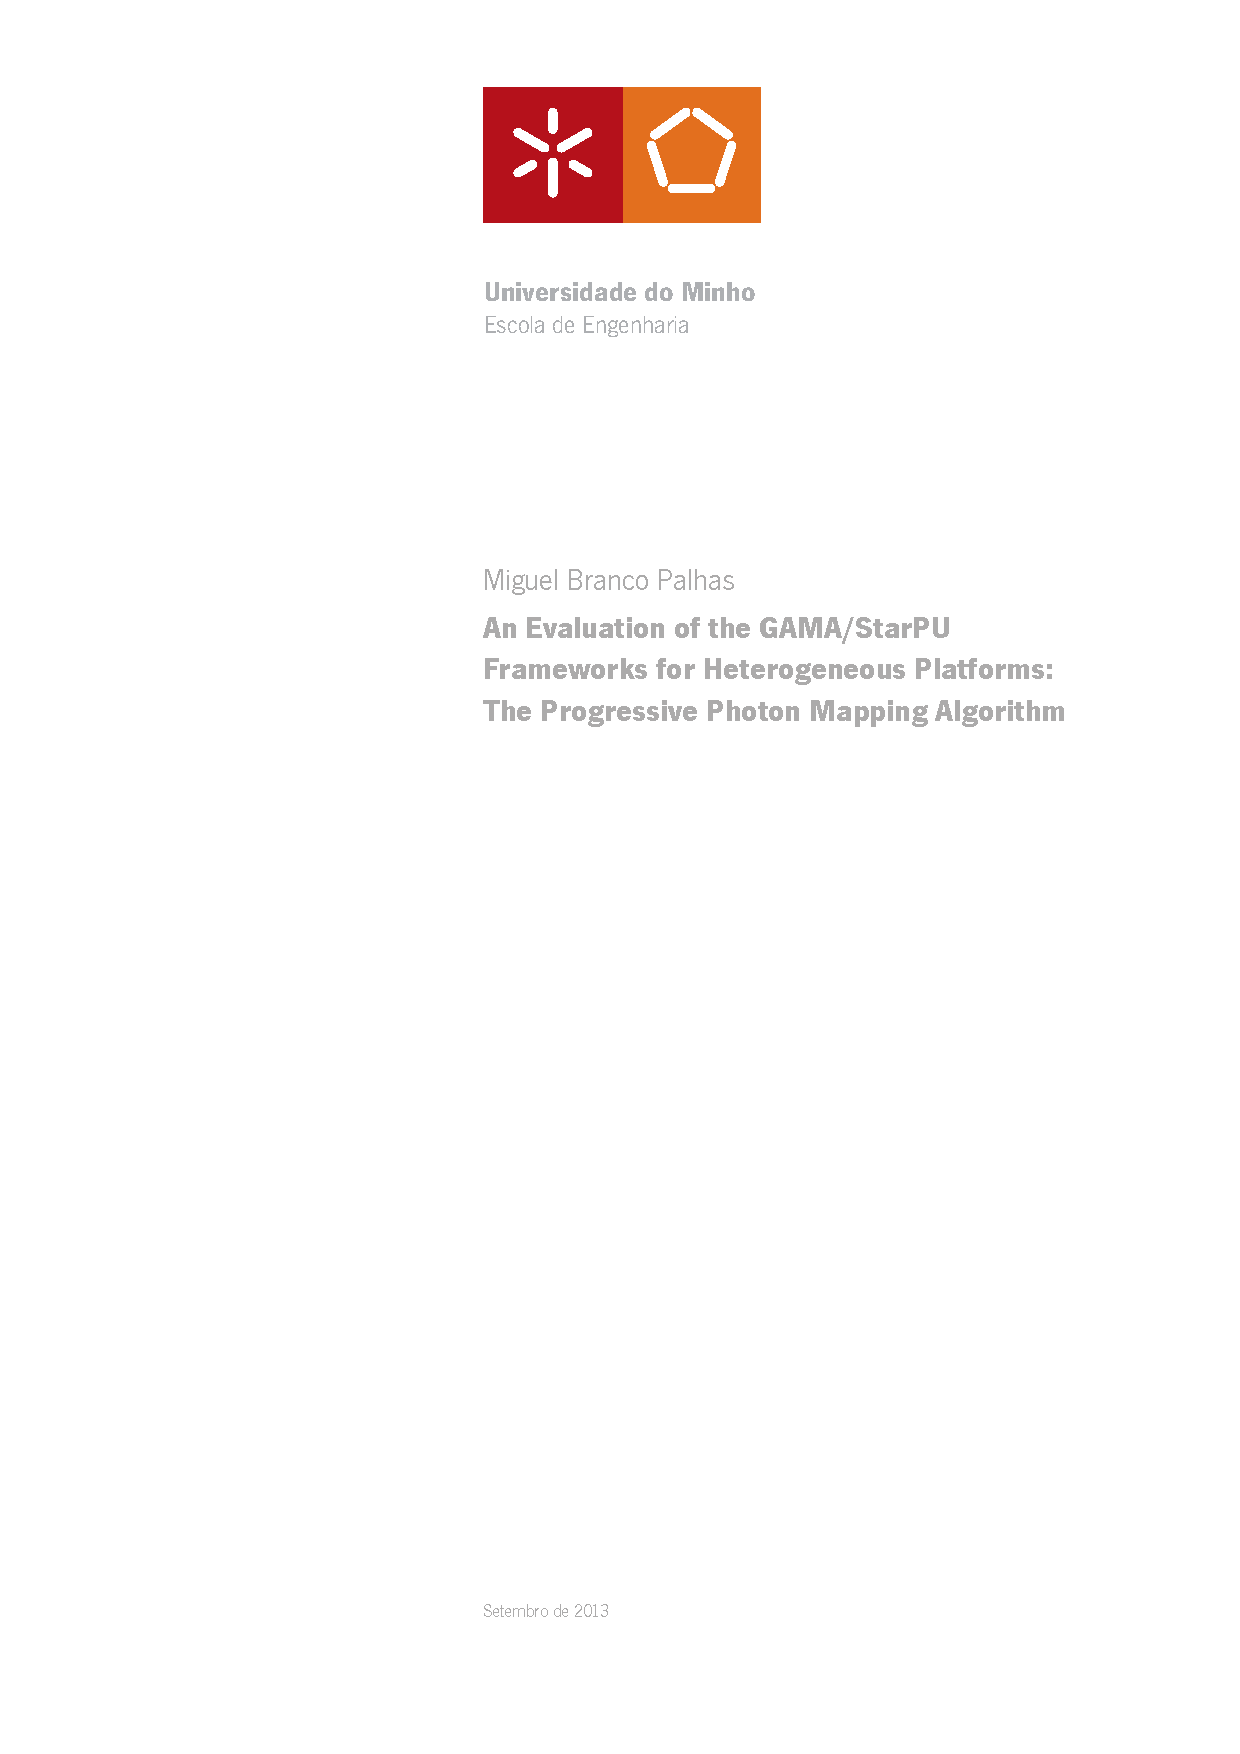
\includepdf[pages=-]{img/cover}

\pagestyle{fancy}
\renewcommand{\headrulewidth}{0.4pt}
\fancyhead[LO,RE]{}
\fancyhead[LE]{\slshape \leftmark}
\fancyhead[RO]{\slshape \rightmark}
\fancyfoot[RO,LE]{\thepage}%
\fancyfoot[C]{}

\fancypagestyle{plain}{%
  \renewcommand{\headrulewidth}{0.0pt}
  \fancyhead{}
  \fancyfoot[C]{}
  \fancyfoot[RO,LE]{\thepage}
}

\frontmatter
\setcounter{page}{3}
\subfile{frontmatter/01_acknowledgments}
\subfile{frontmatter/02_abstract}
\subfile{frontmatter/03_resumo}
\subfile{frontmatter/04_contents}

\cleardoublepage
\pagenumbering{arabic}

\mainmatter
\subfile{tex/100_introduction}
\subfile{tex/200_background}
\subfile{tex/300_gama}
\subfile{tex/400_starpu}
\subfile{tex/500_ppm}
\subfile{tex/600_implementation}
\subfile{tex/700_results}
\subfile{tex/800_conclusions}
\subfile{tex/900_future}
\subfile{tex/999_todo}


\cleardoublepage
\backmatter
\pdfbookmark{References}{references}
%\nocite{*}
\printbibliography
\appendix
\subfile{appendix/A_test_env}
\subfile{appendix/Z_signatures}

\end{document}
